% !TeX TS-program = pdflatex


\documentclass[a4paper]{article}

% \usepackage[default]{fontsetup}

\usepackage{fancyhdr}
\usepackage{extramarks}
\usepackage{amsmath}
\usepackage{amsthm}
\usepackage{amsfonts}
\usepackage{tikz}
\usepackage[plain]{algorithm}
\usepackage{algpseudocode}
\usepackage{enumerate}
\usepackage{tikz}

\usetikzlibrary{automata,positioning}

%
% Basic Document Settings
%  

\topmargin=-0.2in
\evensidemargin=0in
\oddsidemargin=0in
\textwidth=6.5in
\textheight=9.5in
\headsep=0.25in

\linespread{1.1}

\pagestyle{fancy}
\lhead{\hmwkAuthorName}
\chead{\hmwkClass : \hmwkTitle}
\rhead{\firstxmark}
\lfoot{\lastxmark}
\cfoot{\thepage}

\renewcommand\headrulewidth{0.4pt}
\renewcommand\footrulewidth{0.4pt}

\setlength\parindent{0pt}

%
% Create Problem Sections
%

\newcommand{\enterProblemHeader}[1]{
    \nobreak\extramarks{}{Problem \arabic{#1} continued on next page\ldots}\nobreak{}
    \nobreak\extramarks{Problem \arabic{#1} (continued)}{Problem \arabic{#1} continued on next page\ldots}\nobreak{}
}

\newcommand{\exitProblemHeader}[1]{
    \nobreak\extramarks{Problem \arabic{#1} (continued)}{Problem \arabic{#1} continued on next page\ldots}\nobreak{}
    \stepcounter{#1}
    \nobreak\extramarks{Problem \arabic{#1}}{}\nobreak{}
}

\newcommand*\circled[1]{\tikz[baseline=(char.base)]{
		\node[shape=circle,draw,inner sep=2pt] (char) {#1};}}


\setcounter{secnumdepth}{0}
\newcounter{partCounter}
\newcounter{homeworkProblemCounter}
\setcounter{homeworkProblemCounter}{1}
\nobreak\extramarks{Problem \arabic{homeworkProblemCounter}}{}\nobreak{}

%
% Homework Problem Environment
%
% This environment takes an optional argument. When given, it will adjust the
% problem counter. This is useful for when the problems given for your
% assignment aren't sequential. See the last 3 problems of this template for an
% example.
%

\newenvironment{homeworkProblem}[1][-1]{
    \ifnum#1>0
        \setcounter{homeworkProblemCounter}{#1}
    \fi
    \section{Problem \arabic{homeworkProblemCounter}}
    \setcounter{partCounter}{1}
    \enterProblemHeader{homeworkProblemCounter}
}{
    \exitProblemHeader{homeworkProblemCounter}
}

%
% Homework Details
%   - Title
%   - Class
%   - Due date
%   - Name
%   - Student ID

\newcommand{\hmwkTitle}{Homework\ \#10}
\newcommand{\hmwkClass}{Probability \& Statistics for EECS}
\newcommand{\hmwkDueDate}{2024-12-17}
\newcommand{\hmwkAuthorName}{Wenye Xiong}
\newcommand{\hmwkAuthorID}{2023533141}


%
% Title Page
%

\title{
    \vspace{2in}
    \textmd{\textbf{\hmwkClass:\\  \hmwkTitle}}\\
    \normalsize\vspace{0.1in}\small{Due\ on\ \hmwkDueDate\ at 11:59}\\
	\vspace{4in}
}

\author{
	Name: \textbf{\hmwkAuthorName} \\
	Student ID: \hmwkAuthorID}
\date{}

\renewcommand{\part}[1]{\textbf{\large Part \Alph{partCounter}}\stepcounter{partCounter}\\}

%
% Various Helper Commands
%

% Useful for algorithms
\newcommand{\alg}[1]{\textsc{\bfseries \footnotesize #1}}
% For derivatives
\newcommand{\deriv}[1]{\frac{\mathrm{d}}{\mathrm{d}x} (#1)}
% For partial derivatives
\newcommand{\pderiv}[2]{\frac{\partial}{\partial #1} (#2)}
% Integral dx
\newcommand{\dx}{\mathrm{d}x}
% Alias for the Solution section header
\newcommand{\solution}{\textbf{\large Solution}}
% Probability commands: Expectation, Variance, Covariance, Bias
\newcommand{\E}{\mathrm{E}}
\newcommand{\Var}{\mathrm{Var}}
\newcommand{\Cov}{\mathrm{Cov}}
\newcommand{\Bias}{\mathrm{Bias}}

\begin{document}


% \maketitle
% \thispagestyle{empty}
% \pagebreak

\date{
Due on Dec. 17, 2024, 11:59 UTC+8}
\title{SI 140A-02  Probability \& Statistics for EECS, Fall 2024 \\
Homework 10}
\maketitle
Read all the instructions below carefully before you start working on the assignment, and before you make a submission.
\begin{itemize}
    \item You are required to write down all the major steps towards making your conclusions; otherwise you may obtain limited points of the problem.
    \item Write your homework in English; otherwise you will get no points of this homework.
    \item Any form of plagiarism will lead to $0$ point of this homework. 
\end{itemize}
\newpage
\begin{homeworkProblem}[1]
Let $U_{i} \sim \operatorname{Unif}(0,1), i \geq 1$ be i.i.d. random variables. Define $N$ as follows:
$$
N=\max \left\{n: \prod_{i=1}^{n} U_{i} \geq e^{-1}\right\}
$$
\begin{enumerate}[(a)]
\item Estimate $\mathrm{E}(N)$ by generating 5000 samples of $N$ and then use the sample mean.
\item Estimate $\operatorname{Var}(N)$.
\item Estimate $P(N=i)$, for $i=0,1,2,3$.
\item Can you find the exact distribution of $N$ ?
\end{enumerate}
\subsection{Solution}
(a), (b) and (c) can be solved by simulation. You can see the code in the appendix.\\
% filepath: SI140A_02 Homework10.tex
(d) We can find the exact distribution of $N$ as follows:

Let's first transform the problem:
\begin{align*}
    N &= \max\{n: \prod_{i=1}^n U_i \geq e^{-1}\} \\
    &= \max\{n: \sum_{i=1}^n \ln(U_i) \geq -1\}
\end{align*}

Key observations:
\begin{itemize}
    \item If $U \sim \text{Uniform}(0,1)$, then $-\ln(U) \sim \text{Exponential}(1)$
    \item Let $Y_i = -\ln(U_i)$, then $Y_i \sim \text{Exponential}(1)$
    \item Sum of exponential random variables follows Gamma distribution
    \item $S_n = \sum_{i=1}^n Y_i \sim \text{Gamma}(n,1)$
\end{itemize}

Therefore:
\begin{align*}
    P(N = k) &= P(S_k \leq 1 \text{ and } S_{k+1} > 1) \\
    &= P(S_k \leq 1) - P(S_{k+1} \leq 1) \\
    &= \frac{\gamma(k,1)}{\Gamma(k)} - \frac{\gamma(k+1,1)}{\Gamma(k+1)}
\end{align*}

where $\gamma(k,1)$ is the lower incomplete gamma function and $\Gamma(k)$ is the gamma function.

This gives us the exact probability mass function for $N$.

\end{homeworkProblem}

\newpage

\begin{homeworkProblem}[2]
    Visualization of Bivariate Normal Distribution with correlation coefficient $\rho$
    \begin{enumerate}[(a)]
        \item Use the following transformation to generate samples from bivariate Normal distribution with correlation coefficient $\rho$ :
        $$
        \begin{aligned}
        & X=Z \\
        & Y=\rho Z+\sqrt{1-\rho^{2}} W
        \end{aligned}
        $$
        where $-1<\rho<1, Z$ and $W$ are i.i.d. random variables satisfying $\mathcal{N}(0,1)$.
        \item Plot the joint pdf function and the corresponding contour(or isocontour) as the following figure:\\
        \begin{figure*}[htb]
            \centering
            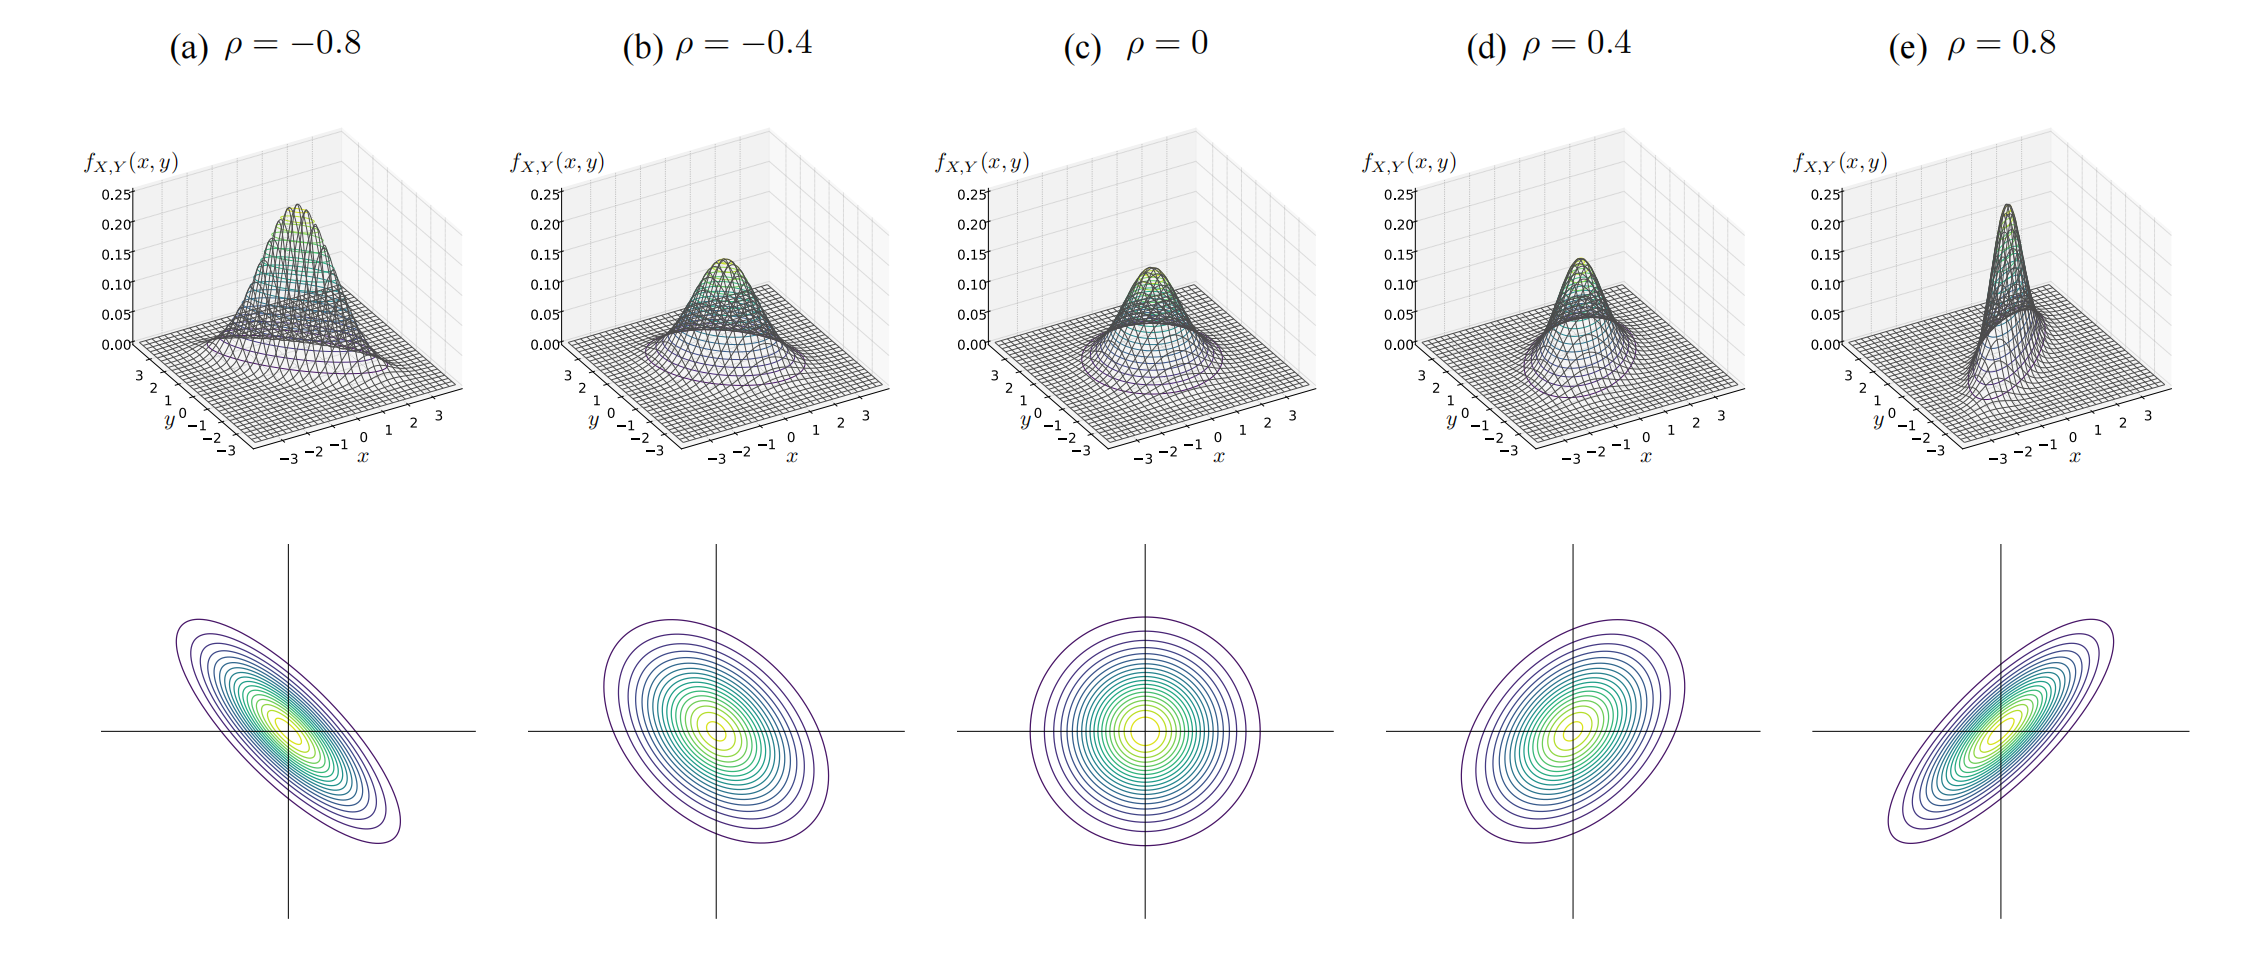
\includegraphics[width=1\linewidth]{图片1.png}
            
        \end{figure*}
    \end{enumerate}
\end{homeworkProblem}
\subsection{Solution}
See the code in the appendix for the implementation of the above problem.\\
\newpage

\begin{homeworkProblem}[3]
     Let $X_{1} \sim \operatorname{Expo}\left(\lambda_{1}\right), X_{2} \sim \operatorname{Expo}\left(\lambda_{2}\right)$ and $X_{3} \sim \operatorname{Expo}\left(\lambda_{3}\right)$ be independent.
     \begin{enumerate}[(a)]
         \item Find $E\left(X_{1} \mid X_{1}>2024\right)$
         \item Find $E\left(X_{1} \mid X_{1}<1997\right)$
         \item Find $E\left(X_{1}+X_{2}+X_{3} \mid X_{1}>1997, X_{2}>2014, X_{3}>2025\right)$ in terms of $\lambda_{1}, \lambda_{2}, \lambda_{3}$.
     \end{enumerate}

     \subsection{Solution}
     (a)\\
     According to the memoryless property of exponential distribution, we have
     \begin{center}
            $E\left(X_{1} \mid X_{1}>2024\right) = 2024 + E\left(X_{1} - 2024 \mid X_1 > 2024\right) = 2024 + E\left(X_{1}\right) = 2024 + \frac{1}{\lambda_1}$
     \end{center}
    (b)\\
    Similarly, we have
    \begin{center}
        $E\left(X_{1} \mid X_{1}<1997\right) = 1997 - E\left(1997 - X_{1} \mid X_1 < 1997\right) = 1997 - E\left(X_{1}\right) = 1997 - \frac{1}{\lambda_1}$
    \end{center}
    (c)\\
    Since $X_1, X_2, X_3$ are independent, we have
    \begin{center}
        $E\left(X_{1}+X_{2}+X_{3} \mid X_{1}>1997, X_{2}>2014, X_{3}>2025\right) = E\left(X_{1} \mid X_{1}>1997\right) + E\left(X_{2} \mid X_{2}>2014\right) + E\left(X_{3} \mid X_{3}>2025\right)$\\
        $= \frac{1}{\lambda_1} + \frac{1}{\lambda_2} + \frac{1}{\lambda_3} + 1997 + 2014 + 2025 = 6036 + \frac{1}{\lambda_1} + \frac{1}{\lambda_2} + \frac{1}{\lambda_3}$
    \end{center}
\end{homeworkProblem}

\newpage

\begin{homeworkProblem}[4]
    Let $X$ and $Y$ be two continuous random variables with joint PDF
$$
f_{X, Y}(x, y)= \begin{cases}6 x y & \text { if } 0 \leq x \leq 1,0 \leq y \leq \sqrt{x} \\ 0 & \text { otherwise }\end{cases}
$$

    \begin{enumerate}[(a)]
        \item Find the marginal distributions of $X$ and $Y$. Are $X$ and $Y$ independent?
        \item Find $E[X \mid Y=y]$ and $\operatorname{Var}[X \mid Y=y]$ for $0 \leq y \leq 1$.
        \item Find $E[X \mid Y]$ and $\operatorname{Var}[X \mid Y]$.
    \end{enumerate}

\subsection{Solution}
(a) The supports of $X$ and $Y$ are both [0,1]. In this way, we have

and

$$\begin{aligned}f_{X}(x)&=\:\int_{-\infty}^{\infty}f_{X,Y}(x,y)dy\\&=\:\int_{0}^{\sqrt{x}}6xydy\\&=\:3xy^{2}\bigg|_{y=0}^{y=\sqrt{x}}\\&=\:3x^{2},\end{aligned}$$
$$\begin{aligned}f_{Y}(y)&=\:\int_{-\infty}^{\infty}f_{X,Y}(x,y)dx\\&=\:\int_{y^{2}}^{1}6xydx\\&=\:3yx^{2}\Big|_{x=y^{2}}^{x=1}\\&=\:3y-3y^{5}.\end{aligned}$$
$$\begin{aligned}&f_{X}(x)=\:\begin{cases}3x^2&\text{if }0\leq x\leq1,\\0&\text{otherwise.}\end{cases}\\&f_{Y}(y)=\:\begin{cases}3y-3y^5&\text{if }0\leq y\leq1,\\0&\text{otherwise.}\end{cases}\end{aligned}$$
Since $f_{X,Y}(x,y)\neq f_{X}(x)f_{Y}(y),X$ and $Y$ are not independent.

Therefore,

$$E[X|Y=y]=\int_{-\infty}^{\infty}xf_{X|Y}(x|y)dx,$$

to calculate $E[X|Y=y]$, we need to first calculate $f_X|Y(x|y).$

If $y^2\leq x\leq1$,

$$f_{X|Y}(x|y)=\frac{f_{X,Y}(x,y)}{f_Y(y)}=\frac{2x}{1-y^4}.$$

In this way,

$$f_{X|Y}(x|y)=\begin{cases}\frac{2x}{1-y^4}&\text{if}y^2\le x\le1,\\0&\text{otherwise.}\end{cases}$$

(b) Since

$$E[X|Y=y]=\int_{-\infty}^{\infty}xf_{X|Y}(x|y)dx,$$

to calculate $E[X|Y=y]$, we need to first calculate $f_X|Y(x|y).$

If $y^2\leq x\leq1$,

$$f_{X|Y}(x|y)=\frac{f_{X,Y}(x,y)}{f_Y(y)}=\frac{2x}{1-y^4}.$$

In this way,

$$f_{X|Y}(x|y)=\begin{cases}\frac{2x}{1-y^4}&\text{if}y^2\le x\le1,\\0&\text{otherwise.}\end{cases}$$\\

Therefore,
$$
\begin{aligned}
E[X \mid Y=y] & =\int_{-\infty}^{\infty} x f_{X \mid Y}(x \mid y) d x \\
& =\int_{y^2}^1 x \frac{2 x}{1-y^4} d x \\
& =\left.\frac{2}{3\left(1-y^4\right)} x^3\right|_{x=y^2} ^{x=1} \\
& =\frac{2\left(1-y^6\right)}{3\left(1-y^4\right)} \\
& =\frac{2}{3} \cdot \frac{1+y^2+y^4}{1+y^2}
\end{aligned}
$$

Since
$$
\operatorname{Var}[X \mid Y=y]=E\left[X^2 \mid Y=y\right]-(E[X \mid Y=y])^2
$$
to calculate $\operatorname{Var}[X \mid Y=y]$, we need to first calculate $E\left[X^2 \mid Y=y\right]$.
Since
$$
\begin{aligned}
E\left[X^2 \mid Y=y\right] & =\int_{-\infty}^{\infty} x^2 f_{X \mid Y}(x \mid y) d x \\
& =\int_{y^2}^1 x^2 \frac{2 x}{1-y^4} d x \\
& =\left.\frac{1}{2\left(1-y^4\right)} x^4\right|_{x=y^2} ^{x=1} \\
& =\frac{1-y^8}{2\left(1-y^4\right)} \\
& =\frac{1+y^4}{2}
\end{aligned}
$$
we have,
$$
\begin{aligned}
\operatorname{Var}[X \mid Y=y] & =E\left[X^2 \mid Y=y\right]-(E[X \mid Y=y])^2 \\
& =\frac{1+y^4}{2}-\left(\frac{2\left(1-y^6\right)}{3\left(1-y^4\right)}\right)^2 \\
& =\frac{1+y^4}{2}-\frac{4}{9} \cdot \frac{\left(1+y^2+y^4\right)^2}{\left(1+y^2\right)^2}
\end{aligned}
$$
(c) According to the result in question(b), we have
$$
\begin{aligned}
& E[X \mid Y]=\frac{2}{3} \cdot \frac{1+Y^2+Y^4}{1+Y^2} \\
& \operatorname{Var}[X \mid Y]=\frac{1+Y^4}{2}-\frac{4}{9} \cdot \frac{\left(1+Y^2+Y^4\right)^2}{\left(1+Y^2\right)^2}
\end{aligned}
$$
\end{homeworkProblem}

\newpage

\begin{homeworkProblem}[5]
    Let $X$ be a discrete r.v. whose distinct possible values are $x_{0}, x_{1}, \ldots$, and let $p_{k}=$ $P\left(X=x_{k}\right)$. The entropy of $X$ is $H(X)=\sum_{k=0}^{\infty} p_{k} \log _{2}\left(1 / p_{k}\right)$.
    \begin{enumerate}[(a)]
        \item Find $H(X)$ for $X \sim \operatorname{Geom}(p)$.
        \item Let $X$ and $Y$ be i.i.d. discrete r.v.s. Show that $P(X=Y) \geq 2^{-H(X)}$.
    \end{enumerate}
\end{homeworkProblem}
\subsection{Solution}
(a)\\ The PMF of $X$ is $P(X=k)=p(1-p)^k$ since there is $X \sim \operatorname{Geom}(p)$. Thus we have
$$
\begin{aligned}
H(X) & =-\sum_{k=0}^{\infty} p(1-p)^k \log _2\left(p(1-p)^k\right) \\
& =-p \sum_{k=0}^{\infty} k(1-p)^k \log _2(1-p)-p \log _2 p \sum_{k=0}^{\infty}(1-p)^k \\
& =-\log _2 p-\frac{1-p}{p} \log _2(1-p)
\end{aligned}
$$\\
(b)\\ Since $X$ and $Y$ are i.i.d random variables, via LOTP, we have
$$
\begin{aligned}
P(X=Y) & =\sum_{k=0}^{\infty} P(X=Y \mid Y=k) \cdot P(Y=k) \\
& =\sum_{k=0}^{\infty} P(X=k) \cdot P(Y=k)=\sum_{k=0}^{\infty} p_k^2
\end{aligned}
$$

Denote $Z$ as a new discrete random variable such that $P\left(Z=p_k\right)=p_k$, then we have:
$$
E(Z)=\sum_{k=0}^{\infty} p_k \times p_k=P(X=Y)
$$

Since $\log (\cdot)$ is a convex function, according to Jensen's inequality, we have $E(\log (Z)) \leq \log (E(Z))$, thus there is
$$
\begin{aligned}
& \sum p_k \log _2 p_k \leq \log _2 \sum p_k^2 \\
\Leftrightarrow & -H(X) \leq \log _2 P(X=Y) \\
\Leftrightarrow & P(X=Y) \geq 2^{-H(X)}
\end{aligned}
$$
\newpage
\begin{homeworkProblem}[6]
    Instead of predicting a single value for the parameter, we give an interval that is likely to contain the parameter: A $1-\delta$ confidence interval for a parameter $p$ is an interval $[\hat{p}-\epsilon, \hat{p}+\epsilon]$ such that ${Pr}(p \in[\hat{p}-\epsilon, \hat{p}+\epsilon]) \geq 1-\delta$. Now we toss a coin with probability $p$ landing heads and probability $1-p$ landing tails. The parameter $p$ is unknown and we need to estimate its value from experiment results. We toss such coin $N$ times. Let $X_{i}=1$ if the $i$ th result is head, otherwise 0 . We estimate $p$ by using

$$
\hat{p}=\frac{X_{1}+\ldots+X_{N}}{N}
$$

Find the $1-\delta$ confidence interval for $p$, then discuss the impacts of $\delta$ and $N$.
\begin{enumerate}[(a)]
    \item  Method 1: Adopt Chebyshev inequality to find the $1-\delta$ confidence interval for $p$, then discuss the impacts of $\delta$ and $N$.
    \item Method 2: Adopt Hoeffding bound to find the $1-\delta$ confidence interval for $p$, then discuss the impacts of $\delta$ and $N$.
    \item Discuss the pros and cons of the above two methods.
\end{enumerate}
\subsection{Solution}
Since $X_i \sim \operatorname{Bern}(p), X_i \in\{0,1\}$, we have $\mathbb{E}\left[X_i\right]=p$ and $\mathbb{V}\left[X_i\right]=p(1-p)$. Therefore, we have
$$
\mathbb{E}[\hat{p}]=p, \mathbb{V}[\hat{p}]=\frac{p(1-p)}{N}
$$

Besides, we know that
$$
P(p \in[\hat{p}-\varepsilon, \hat{p}+\varepsilon]) \geq 1-\delta \Leftrightarrow P(|\hat{p}-p| \geq \varepsilon) \leq \delta
$$\\
(a)\\ Applying Chebyshev's inequality on random variable $\hat{p}$, we have
$$
P(|\hat{p}-p| \geq \epsilon) \leq \frac{p(1-p)}{N \epsilon^2} \Rightarrow \delta=\frac{p(1-p)}{N \epsilon^2}, \epsilon=\sqrt{\frac{p(1-p)}{N \delta}}
$$

Therefore, we know that $\delta$ negatively correlates with $\epsilon$, i.e., given a fixed number of samples $N$, there is natural trade-off between accuracy and confidence. Besides, 1) Fix the confidence interval parametrized by $\delta$, reducing the estimation error $\epsilon$ requires increasing the number of samples $N$. 2) Fix the estimation error $\epsilon$, narrowing the confidence interval requires increasing the number of samples $N$. That is, the impacts of $N$ is on both the "estimation accuracy" and "estimation confidence".
\\(b)\\ Applying Hoeffding's inequality on random variable $\hat{p}$, we have
$$
P(|\hat{p}-p| \geq \epsilon) \leq 2 e^{-2 N \epsilon^2} \Rightarrow \delta=2 e^{-2 N \epsilon^2}, \epsilon=\sqrt{\frac{\ln (2 / \delta)}{2 N}}
$$

The effects of $\delta$ and $N$ are similarly discussed as in (a).
\\(c)\\ Chebyshev's inequality \\
- Pros: 1) sharp bound and cannot be improved in general. 2) can be improved with extra distributional information on polynomial moments.\\
- Cons: 1) requires the existence of moments until the second order. 2) quadratic convergence rate.

Hoeffding's inequality\\
- Pros: 1) exponential convergence rate. 2) does not require assumption on moments.\\
- Cons: 1) works only for sub-Gaussian . 2) in general not sharp when the variance is small.
\end{homeworkProblem}

\newpage
\begin{homeworkProblem}[7](\textbf{Optional Challenging Problem})
    We consider the progressive Monty Hall problem. This time we assume there are $n$ identical doors, where $n$ is an integer satisfying $n \geq 3$. One door conceals a car, the other $n-1$ doors conceal goats. You choose one of the doors at random but do not open it. Monty then opens a door he knows to conceal a goat, always choosing randomly among the available doors. At this point he gives you the option either of sticking with your original door or switching to one of the remaining doors. You make your decision. Monty now eliminates another goat-concealing door (at random) and once more gives you the choice either of sticking or switching. This process continues until only two doors remain in play. What strategy should you follow to maximize your chances of winning? We consider three strategies: (1) Select a door at random and stick with it throughout. (2) Select a door at random, then switch doors at every opportunity, choosing your door randomly at each step. (3) Select a door at random, stick with your first choice until only two doors remain, and then switch. When $n=10$ and $n=1000$, \textbf{please run simulations to estimate the winning probability of each strategy. Check which strategy is best and provide the corresponding intuition.}
\end{homeworkProblem}


\end{document}